% The use of phonetic motor invariants can improve automatic phoneme discrimination
% Castellini, Metta, Fadiga, Badino
% submitted to PNAS

\documentclass{pnastwo}

% ---------------------------------- bookkeeping

% remove for submission
\usepackage[dvips]{graphicx}

%\usepackage{pnastwoF}
\usepackage{amssymb}
\usepackage{amsfonts}
\usepackage{amsmath}

\newcommand{\lio}{\textsf{lio}}
\newcommand{\ttu}{\textsf{ttu}}
\newcommand{\vlio}{\textsf{vlio}}
\newcommand{\vttu}{\textsf{vttu}}
\newcommand{\alio}{\textsf{alio}}
\newcommand{\attu}{\textsf{attu}}

\newcommand{\overall}{\emph{overall}}
\newcommand{\spka}{\emph{spk5vs1}}
\newcommand{\spkb}{\emph{spk3vs3}}
\newcommand{\spkc}{\emph{spk1vs5}}
\newcommand{\coa}{\emph{coart4vs1}}
\newcommand{\cob}{\emph{coart3vs2}}

%%%%%%%%%%%%%%%%%%%%%%%%%%%%%%
%% Don't type in anything in the following section:
%%%%%%%%%%%%
%% For PNAS Only:
\contributor{Submitted to Proceedings
of the National Academy of Sciences of the United States of America}
\url{www.pnas.org/cgi/doi/10.1073/pnas.0709640104}
\copyrightyear{2008}
\issuedate{Issue Date}
\volume{Volume}
\issuenumber{Issue Number}
%%%%%%%%%%%%

\begin{document}

% ---------------------------------- frontmatter

\title{The use of phonetic motor invariants\\
can improve automatic phoneme discrimination}

\author{
Claudio Castellini\affil{1}{German Aerospace Research Center, Oberpfaffenhofen, Germany},
Giorgio Metta\affil{2}{Italian Institute of Technology, Genova, Italy},
Luciano Fadiga\affil{3}{DSBTA, University of Ferrara, Italy} and
Leonardo Badino\affil{2}{}
}

\contributor{Submitted to Proceedings of the National Academy of Sciences
of the United States of America}

\maketitle

\begin{article}

\begin{abstract}

  We hereby investigate the use of phonetic motor invariants (MIs),
  that is, recurring kinematic patterns of the human phonetic articulators,
  to improve automatic phoneme discrimination. Using a multi-subject
  database of synchronized speech and lips/tongue trajectories, we first
  identify MIs commonly associated with bilabial and dental consonants,
  and use them to simultaneously segment speech and motor signals.
  We then build a simple neural network-based regression schema (an Audio-Motor
  Map, AMM) mapping audio features of these segments to the corresponding
  MIs.
  
  Extensive experimental results show that
  $(a)$ $16$ simple features extracted from the MIs, as originally gathered from
    articulatory sensors, are dramatically more effective than $390$ state-of-the-art
    audio features, in automatically discriminating bilabials from dentals;
  $(b)$ the same features, reconstructed using the AMM, are in general as effective
    as the audio features, and sometimes better when used together with them.
    These claims are shown to hold in ideal training conditions (noise-free,
    large multi-subject training set) as well as when training on a subset of the
    speakers, and on a subset of the coarticulating phonemes.
    
  Lastly, we show that the AMM-reconstructed motor features alone are dramatically
  more resilient to noise than the audio features.
  
  These results support some of the claims of the motor theory of speech perception
  and add experimental evidence of the actual utility of MIs in the more general
  framework of automated speech recognition.
  
% even if we compare against
%  a state-of-the-art audio feature set which is about $20$ times larger than
 % that extracted from MIs. These results encourage the use of MIs in the more
 % general framework of automated speech recognition. Moreover, our findings 
 % support some of the claims of the motor theory of speech perception.

\end{abstract}

\keywords{motor theory of speech | machine learning | phoneme discrimination | speech recognition}

% ---------------------------------- the paper

Active prosthetic hands, driven by a motor to open and close the
``claw,'' have been around for many years.  Recently, however,
advances in mechatronics have improved such hands and currently
various prosthetic hands with 3 or more active degrees of freedom are
being put on the market.  Such hand developments are a result of
various robotic hands which are highly humanoid, light and gifted with
a number of degrees of freedom. Attempts in this sense include, e.g.,
the DLR prosthetic hand (\cite{Hua2006}---see Figure
\ref{fig:DLRHandII}), the CyberHand project \cite{cyberhand}, and the
i-LIMB hand by Touch Bionics \cite{ilimb}.

\begin{figure}
  \begin{tabular}{cc}
    \includegraphics[height=0.12\textheight]{figs/DLRHand-Ball-comp.jpg} &
    \includegraphics[height=0.12\textheight]{figs/DLR-Prothese.jpg}
  \end{tabular}
  \caption{(left) The DLR Hand II. (right) The DLR prosthetic hand.}
  \label{fig:DLRHandII}
\end{figure}

Still, a general sense of frustration impends, as far as
\emph{control} of the prosthesis is concerned. As a matter of fact,
given the current state of the art, it is basically impossible for the
patient to precisely command the prosthesis what to do; whereas,
operating a hand requires a fine control down to the level of the
single fingers. First of all, presented with a certain task such as
turning a door handle or grabbing a car key, the patient must be able
to enforce the correct grasping type; this involves the activation of
some joints only, and in particular positions. Secondly, the amount of
force involved in the grasp must be controlled, so that it is possible
to grab, e.g., both a hammer without letting it slip and an egg
without breaking it.

To this end, two types of interfaces between the patient and the
prosthesis have been developed or are being studied: \emph{invasive}
and \emph{non-invasive}. The former gather control signals directly
from the user's nervous system, either via brain implants or surgical
use of electrodes. Quite obviously, invasive interfaces are supposed
to deliver a high signal quality, since the signals can be gathered
exactly in the right spots; but they involve surgery and all related
sterility (and psychological) issues. On the other hand, non-invasive
interfaces are easier to handle, manufacture and implant, but require
a much better signal conditioning, since they usually work with
surface (skin) signals or vision and gaze tracking.

In the context of non-invasive interfaces for controlling mechanical
hands, a concrete possibility arises from \emph{forearm surface
electromyography} (EMG), a technique by which muscle
activation potentials are gathered by electrodes placed on the
patient's forearm skin; these potentials can be used to track which
muscles the patient is willing to activate, and with what force.
Surface EMG is therefore, in principle, a cheap and easy way of
detecting what the patient wants the prosthesis to do.

Still, the EMG signal suffers from a number of problems, among which
the unprecise placement of the electrodes, signal drifting and change
due to sweat formation and muscular fatigue and cross-talking among
deep and superficial muscles. It seems, though, that good results can
be obtained via \emph{machine learning} techniques, as shown in, e.g.,
\cite{smagt}. In machine learning, one tries to approximate an unknown
function given its values in a number of samples; the application to
the current problem is exactly that of building a map relating EMG
activation potentials and muscle force, and therefore hand finger
movements.

Such a system must be highly adaptive, accurate and fast---possibly,
able to run in real time, as the patient is wearing the prosthesis.
Another very desirable characteristic is that the system should learn
automatically as the patient moves, being able to understand when new
portions of the input space are being explored, i.e., what new
movements are required of the prosthesis. But so far machine learning
applied to surface EMG has only been able to classify hand postures.
For example, the surface EMG signal can be used to detect whether the
patient is attempting a cylindric grasp or a two-finger grip
\cite{ekvall}; but no indication about the amount of force involved in
the grasping act is detected.

In this paper we show a rather detailed analysis of what machine
learning can do when applied to such a problem. Over several days, we have
gathered forearm surface EMG data while an able-bodied human subject
was gripping in four distinct ways a force sensor; we have then
trained three different machine learning systems to guess, from the
EMG signal,
\begin{enumerate}

  \item what kind of grasp the subject was doing, e.g., thumb and
    index finger, thumb and middle finger, thumb and ring finger or
    thumb and all other fingers; and

  \item how much force the subject was exerting, in order to
    understand whether the grasp was, e.g., a power grasp or rather a
    precision grip. Surprisingly, as far as we know, nobody has ever
    attempted so far to solve this problem, although it is well-known
    that the EMG is related to the force a muscle is exerting.

\end{enumerate}

The three approaches we have experimented with are:
(a) a simple feed-forward neural network with one hidden layer,
(b) a Support Vector Machine with radial basis function kernel
\cite{BGV92}, and (c) Locally Weighted Projection Regression
\cite{lwpr}. Our analysis consists of a preliminary phase in which
several models have been built in a batch fashion, in order to
understand how to deal with the non-stationarity of EMG. The most
interesting challenge has been how to filter out unwanted data, at the
same time keeping a high overall accuracy, both in classification and
regression. Later on, based upon the results obtained in the
preliminary phase, we have developed a simple but effective procedure
for selecting a subset of the samples on-the-fly, called \emph{Online
Uniformisation} (OU).

OU is based upon the simple idea of keeping a minimum inter-sample
Euclidean distance, in order to uniformly sample the input space. The
selected samples are then used to periodically re-train the system,
and check that it has adapted to the new data. The training sets thus
obtained are remarkably small and thus usable on-line, and they offer
an excellent trade-off between size and accuracy. In particular, as a
certain parameter is increased, the size of the uniform training sets
decreases polynomially, while the error rate increases only
linearly; therefore one can obtain much smaller training sets (which
means faster or more adaptive machines) by accepting an error rate
which is only linearly worse.

This behaviour appears in both problems highlighted above (the former
involving classification, the latter regression), and for all the
approaches tested. Our numerical results indicate that, in such a
scenario, the type of grasp can be reconstructed with an average
accuracy of $89.67\% \pm 1.53\%$, and the applied force can be
predicted with an average percentage error of $7.89\% \pm 0.09\%$,
meaning $4.5$N over a range of about $57$N.

The paper is structured as follows: after a brief review of relevant
literature, we describe in detail the experiment and the methods used
to tackle it (Section \ref{sec:m&ms}); then we show and comment on the
experimental results, both the preliminary phase and the online
experiments (Section \ref{sec:exp}); lastly, discussion and
conclusions are presented.

\section{Data set}
\label{sec:dataset}

We work with a a subset of the Contact / Linguometer data
set \cite{tavella}. The data collection setup includes a
\emph{Laryngograph Microprocessor} device (Laryngograph Ltd.,
London \cite{...}) able to gather the speech audio signal
and the electroglottographic (EGG) signal at $16$KHz sampling
rate, and an AG500 electromagnetic articulograph (Carstens
Medizinelektronik GmbH, Germany \cite{...}) able to
record at a sampling rate of $200$Hz the 3D positions of a set
of sensors glued on the tongue, lips and front teeth during
speech production.

The data have been obtained from $6$ female subjects, Italian
mothertongue, while uttering Italian words and pseudo-words,
some of which in interrogative tone. Words were mainly
stress-initial, e.g., /matto/, /nome/, /strada/ (mad, name,
road), and were chosen in order to have several consonants
both at the beginning and in the middle of words, followed
by different vowels and consonants.

The data subset used in this work comprises $77$ words among
those of the Contact / Linguometer data set, namely those containing
/b/, /p/, /d/ or /t/.

\section{The Audio-Motor-Map}
\label{sec:rec}

\subsection{Training the AMM}
\label{subsec:amm_setup}

The procedure for building the AMM closely follows that outlined in previous
literature \cite{papcun,richmond,richmond2007} where a multi-layer perceptron
neural network was employed to reconstruct articulators' positions from an
audio stream. More in detail, the speech spectrogram was there used to predict,
instant by instant, the position of the articulators of interest. Here we apply
a similar approach to reconstruct the velocity and accelerations of \lio\ and \ttu,
in order to avoid as much as possible taking into account physical differences
among subjects (e.g., the width of the mouth, etc.).

For each of the $1157$ audio sequences, the spectrogram is evaluated
over $20$-milliseconds long Hamming windows (slices), using a $20$-filter
Mel-scale filterbank between $20$Hz and $2$KHz. Each slice overlaps by $10$ milliseconds with
the preceding slice. Each single sample of \vlio, \alio, \vttu\ and \attu\ is
then associated to $19$ surrounding spectrogram slices, covering
about $200$ milliseconds of speech and centered around the sample itself. With this
"sliding spectrogram window" method, the four trajectories are completely reconstructed.
The Mel filters, the spectrogram and (later on) the cepstral coefficients of the audio
signal are extracted using the off-the-shelf speech recognition Matlab package
\emph{Voicebox} \cite{Brookes1997}.

About $15000$ samples are extracted from the original $1157$
audio/motor sequences; each input sample consists of $19\cdot 20 = 380$ real
numbers, while the output space is given by the $4$ trajectory points of
the motor signals. A feed-forward neural network is set up in order to
build the AMM, with $380$ input units, one hidden layer with $15$ units and
$4$ output units; the net is trained via the Scaled Conjugate Gradient
Descent method \cite{MOLLER93} and the activation is a logistic sigmoidal function.

Training is done via early stopping on the appropriate validation set (see the previous
Section for the details about CV). This procedure is repeated over $10$ random restarts, and then
the network with best average performance over the $4$ output dimensions is stored.
The performance measure is Matlab's embedded mean-square-error with regularisation
function, in which after some initial experiments we set the regularisation
parameter at $0.714$. This value, as well as all other parameters, have been found in
an initial experimentation phase, by slightly altering values suggested in literature
and/or in the Matlab manual.

No sample normalisation is performed, in order to preserve the time structure of the
spectrogram windows. Targets are normalised in order to lie within the range $[0.1,0.9]$,
since the logistic activation function has asymptotic values of $0$ and $1$.

\subsection{Evaluating the AMM}
\label{subsec:amm_results}

Figure \ref{fig:amm_perf} shows a quantitative assessment of the performance
of the AMM. The measure of performance is the NRMSE (Normalized Root Mean Square Error),
where the normalisation is over the range of each testing data set. The NRMSE
ranges from $16.17\% \pm 0.79\%$ (\vlio, \coa) to $8.22\% \pm 0.58\%$ (\vttu, \spkc).
Regression upon \vlio\ shows the largest error overall. Moreover, the error is on average
larger for the per-coarticulation CV schemas.

Although these figures do not really indicate whether AMM-reconstructed MIs will be
effective in phoneme discrimination, they show that the error rate in regression has
limited magnitude and does not differ dramatically across CV schemas and output signals.
Qualitative inspection of the results (one example is given in Figure \ref{fig:example})
shows that the AMM-reconstructed motor signals are on average rather
similar to the real ones, at least as far as the range of values is concerned.

A definite trend is apparent, favouring the reconstruction of \vlio\ over \vttu\ when
bilabials are presented to the AMM and vice-versa; the trend is numerically confirmed
by checking the Pearson correlation coefficient between AMM-reconstructed and real MIs
according to whether labials (/b/,/p/) or dentals (/d/,/t/) are presented as input
to the AMM. As one can see in Figure \ref{fig:DD}, when the \overall\ CV schema is used,
a ``double dissociation'' pattern appears when comparing the correlation coefficients of
\vlio\ and \vttu\ AMM-reconstructed from labials or dentals
($0.8869 \pm 0.0113$ versus $0.5523 \pm 0.0240$ with Student's t-test $p<0.01$ for \vlio, and
 $0.9276 \pm 0.0096$ versus $0.3307 \pm 0.0278$, $p<0.01$, for \vttu).
In other words, when the AMM
``hears'' /b/ or /p/, it reconstruct effectively the trajectory of the lips, but less
reliably that of the tongue tip; and dually, it reconstructs better the latter one when
presented with /d/ or /t/. This pattern is repeated to an almost uniform extent when the
other CV schemas are used, and also when \alio\ and \attu\ are checked.

\section{Phoneme discrimination}
\label{sec:class}

\subsection{Experiment 1}
\label{subsec:exp1}

In the first experiment the performance of a standard classifier is evaluated
according to the \overall\ CV schema for four different sets of features.
Figure \ref{fig:class1_perf} shows the results.

``Audio'' is a set of $20$ cepstral coefficients evaluated according to the
Mel scale over a bandwidth of $20$Hz to $2$KHz. This is a standard set of features
according to state-of-the-art literature, when the segment
length is fixed a priori. In this case the segment length is not fixed so the
cepstra are evaluated over the whole window, regardless of its length.

``Real motor'' is a set of $17$ coefficients evaluated as follows: for each
signal considered (\vlio, \alio, \vttu\ and \attu), a least-squares cubic fit
is generated over the selected segment, that is, from $t_{start}$ to $t_{end}$
as defined above. This results in $4$ real numbers
per signal, which qualitatively encode the shape of the signal considered. The
$17$th number is the average of the voicing signal over the selected segment.

``Reconstructed motor'' refers to the same procedure as above, but applied
to the AMM-reconstructed signal curves.

Lastly, ``Joint'' denotes a decision procedure obtained by multiplying the
label probabilities obtained from the best classifiers for the audio and
reconstructed motor features.

The classifier is a Support Vector Machine \cite{BGV92} with Gaussian kernel
and hyperparameters $C, \sigma$ found by grid-search. Samples are normalised
by subtracting the mean values and dividing by the standard deviations,
dimension-wise.

The accuracies obtained are, in turn,
$87.64\% \pm 1.05\%$
$92.05\% \pm 0.70\%$
$87.38\% \pm 0.83\%$
$92.65\% \pm 1.00\%$, with statistically significant difference (Student's t-test,
$p<0.01$) between audio and real motor features, audio and joint features, and
reconstructed motor and joint features.

\subsection{Experiment 2}
\label{subsec:exp2}

Experiment 1 was replicated using this time the remaining CV schemas.
Figure \ref{fig:class2_perf} shows the results. (For comparison,
the Figure also shows in the first column the accuracies obtained for
experiment $1$.)

For each and every CV schema, the statistically significant differences seen in
Figure \ref{fig:class1_perf} are present (again, tested via $p$-values);
in particular, in the per-speaker CV schemas, the audio features versus
the joint models show accuracies of
$81.92\% \pm 2.04\%$ and $87.27\% \pm 1.17\%$ (\spka),
$78.90\% \pm 0.61\%$ and $85.74\% \pm 0.44\%$ (\spkb), and
$70.29\% \pm 0.73\%$ and $76.25\% \pm 1.53\%$ (\spkc).

In the per-coarticulation results the gap is more evident; the joint models
here perform worse than the reconstructed motor features. Audio features
versus reconstructed motor features show accuracies of
$41.60\% \pm 9.72\%$ and $62\% \pm 4.86\%$ (\coa) and
$34.84\% \pm 3.64\%$ and $55\% \pm 5.5\%$ (\cob).

\subsection{Experiment 3}
\label{subsec:exp3}

Lastly, for experiment 3 we replaced the audio features with
a $351$-dimensional set of $20$ mel-cepstral
coefficient, this time obtaining by taking $19$ slices of $20$ milliseconds each,
shifted over the audio segment by the required amount of time. This set of
features was compared, again, with the real and reconstructed motor features and
a probabilistic joint model, as white noise was added to the audio signals.

The intensity of noise was let range from nil to $150\%$ of the standard deviation
of each utterance considered; for each sample, $10$ noisy ones were generated, in
order to obtain a larger statistical basis. As in experiment $1$, the \overall\ CV
schema was chosen. Figure \ref{fig:class3_perf} shows the results.

(Notice that the real motor features are not affected by noise.) Student's t-test
reveals that the cepstra-2KHz and joint features are always significantly different.
The cepstra-2KHz and joint features show accuracies ranging from
$91.96\% \pm 0.22\%$ and $93.26\% \pm 0.25\%$ for no noise, to
$69.34\% \pm 0.47\%$ and $75.69\% \pm 0.53\%$ for maximum noise.

\section{Discussion}
\label{sec:disc}

The experiments presented in this paper were inspired by the intuition that the
proficiency of humans in speech recognition is grounded in the interaction
between production and understanding of speech in the human brain. Alvin
Liberman's motor theory of speech perception, although controversial and
recently reviewed and revised \cite{liberman1,liberman2,galant,massaro},
provides a theoretical framework to this intuition, which recent neurological
evidence \cite{dausilio} supports even further.

Assuming this idea as a working hypothesis, we have first tried to identify
a new, biologically inspired, way to segment the audio signal. It is nowadays
widely accepted that this task is impossible by just looking at a standard
speech signal, since the same phoneme has different audio characteristics
depending on the speaker, the voice pitch / speed / accent, and due to the
phenomenon of coarticulation. But physiology tells us that there actually \emph{is} an invariant
over all possible /b/s, for instance, and that is the act that produced it,
that is, a labial plosion. Therefore we propose to segment the audio signal
using the articulators' trajectories to detect
the beginning and end of phonemes. The choice of the articulators and the
conditions on the trajectories are established according to basic rules of
the phonetic production; for example, a /b/ will be identifed from
the beginning to the end of an associated labial plosion. This is possible,
in our case, thanks to a database of synchronised speech / articulographic
data gathered from several human subjects.

With respect to the traditional speech segmentation, done via uniform time
windows of about $20$ milliseconds, this approach focusses on the \emph{act}
that produced the sound. If it is true that speech acts are invariant across
subjects and words, then it should be possible to extract directly from the motor data
fetaures that are more robust to changes in noise, speakers,
coarticulation, etc., than standard
audio features. We use to this end the coeffcients of a cubic fit of the
motor trajectories, so to obtain a qualitative representation of the speech
act.

%
% Giorgio: the cubic fit is not mentioned earlier in the paper?
%

It is clearly shown by our results (Figures \ref{fig:class1_perf}
and \ref{fig:class2_perf}) that these features perform
better than a set of $20$ cepstral coefficients evaluated across each utterance,
while discriminating /b/, /p/, /d/ or /t/ in the database. This gap is even
more evident if examined from a per-speaker or per-coarticulation perspective.
In these tasks, the audio features show a dramatically decreasing discrimination
ability, which is not the case with the motor features. In short, motor features
are ``more invariant'' than audio features across speakers and coarticulations.
This agrees with the motor theory of speech perception.

Now, speech acts are not available in real life --- according to the mirror
paradigm, human beings reconstruct them from the audio signal, after a long
training which begins in infanthood and probably never ends. The AMM is a
representative of this mechanism. Its numerical evaluation
reveals that the normalised root-mean-square-error obtained is rather
uniform across the reconstructed signals, and is at worst $15.55\%$. These
results are coherent with those presented in \cite{papcun,richmond2002,richmond2007}.
But what is more interesting is that the AMM reconstructs labial trajectories
better than dental trajectories when presented with labials and viceversa,
and dually for tongue/dental trajectories and dentals, giving rise to a double
dissociation. A simple explanation of this fact is that human beings
(upon whose data the AMM is trained) identify phonetic actuators which produced
the sound they hear, and neglect the others.

The AMM is used to reconstruct the speech acts from the audio signal; these
reconstructed motor trajectories are then used as input to the phoneme
discrimination classifiers used in the previous experiments. The results
(consider Figures \ref{fig:class1_perf} and \ref{fig:class2_perf} again)
obviously show that they attain lower performances than the features
extracted from the real motor signals, but actually, comparable
to the audio features; and that if we join the audio classification model
to the one obtained for these features (with a trivial probabilistic calculation)
we again obtain a high performance, superior to that of audio features alone
and comaprable to that of real motor features.

AMM-reconstructed audio features also help in the presence of noise. This time
we evaluate the performance of a $200$ milliseconds wide Mel cesptrogram (a total
of $351$ numbers, each one coding \emph{one} phoneme) as noise is added to the
speech signal; the performance degrades steadily. But again, if we join this
model with one obtained by running the AMM on the noisy speech, we uniformly
and significantly increase the performance (Figure \ref{fig:class3_perf}). The
gap seems to widen as more and more noise is added, although this claim would
require a deeper analysis.

Of course, AMM-reconstructed motor features do not carry any more information
(in the sense defined by Shannon) than what is in the speech signal; therefore,
from the point of view of machine learning / speech recognition, one can see
this technique as ``just'' a better way of extracting invariant features from
speech.

\section{Conclusions}
\label{sec:concl}

Although applied to a simple problem like phoneme discrimination, and on a
limited data set, the ideas presented in this paper seem promising and foster
the use of acoustic motor invariants in speech recognition. Also,
the results we present support some of the claims of the motor theory
of speech perception; namely, that speech acts are the real invariant
quantities over speech; and that the phenomenon of coarticulation cannot
be avoided if not resorting to motor-based features.






\begin{acknowledgments}
  This work is supported by the EU-funded projects
  Contact (NEST 5010) and Poeticon (ICT-FP7-215843).
\end{acknowledgments}

% ---------------------------------- refs

% for the submission: comment out the line below, and then include the .bbl
\bibliographystyle{plain} \bibliography{paper}
%\begin{thebibliography}
%...
%\end{thebibliography}

\end{article}

% ---------------------------------- figures & tables

\begin{figure*}[t]
  \centerline{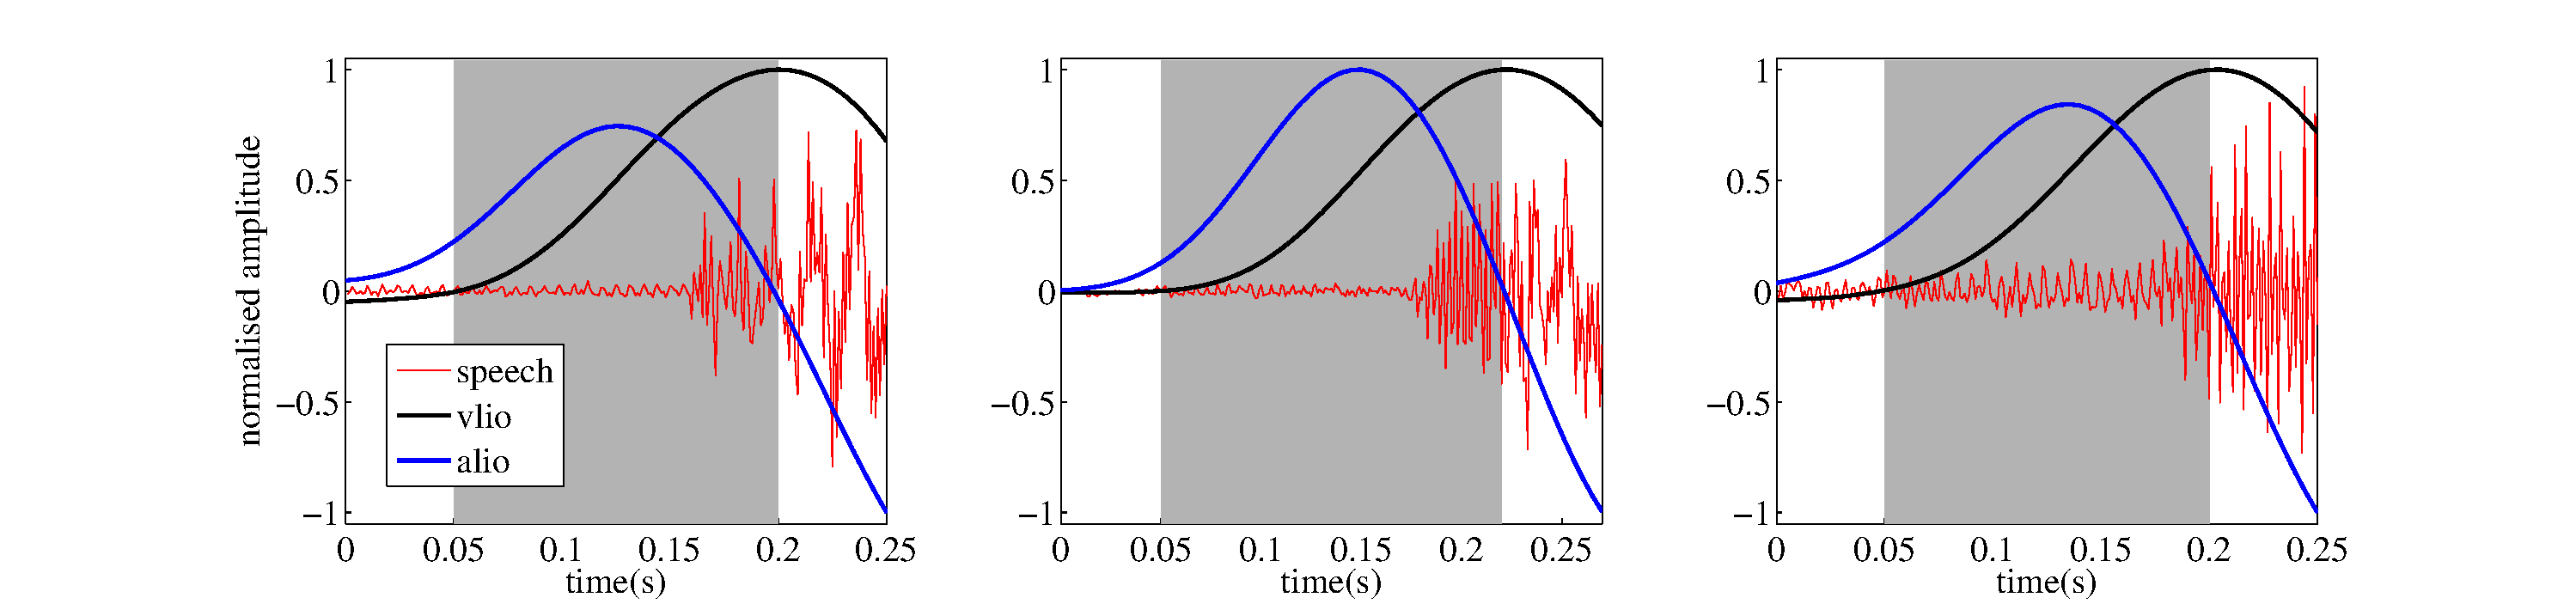
\includegraphics[width=\textwidth]{figs/samples}}
  \caption{The speech signal and motor trajectories of lips opening
    velocity (\vlio) and acceleration (\alio) during utterances containing /b/.
    Left to right: /ba/, subject $5$; /ba/, subject $2$; and /bufalo/, subject $5$.
    The gray zone denotes the detected start and ending of the plosion. All signals
    are normalised over the indicated time frame, for visualisation purposes.}
  \label{fig:isdView}
\end{figure*}

\begin{figure*}[t]
  \centerline{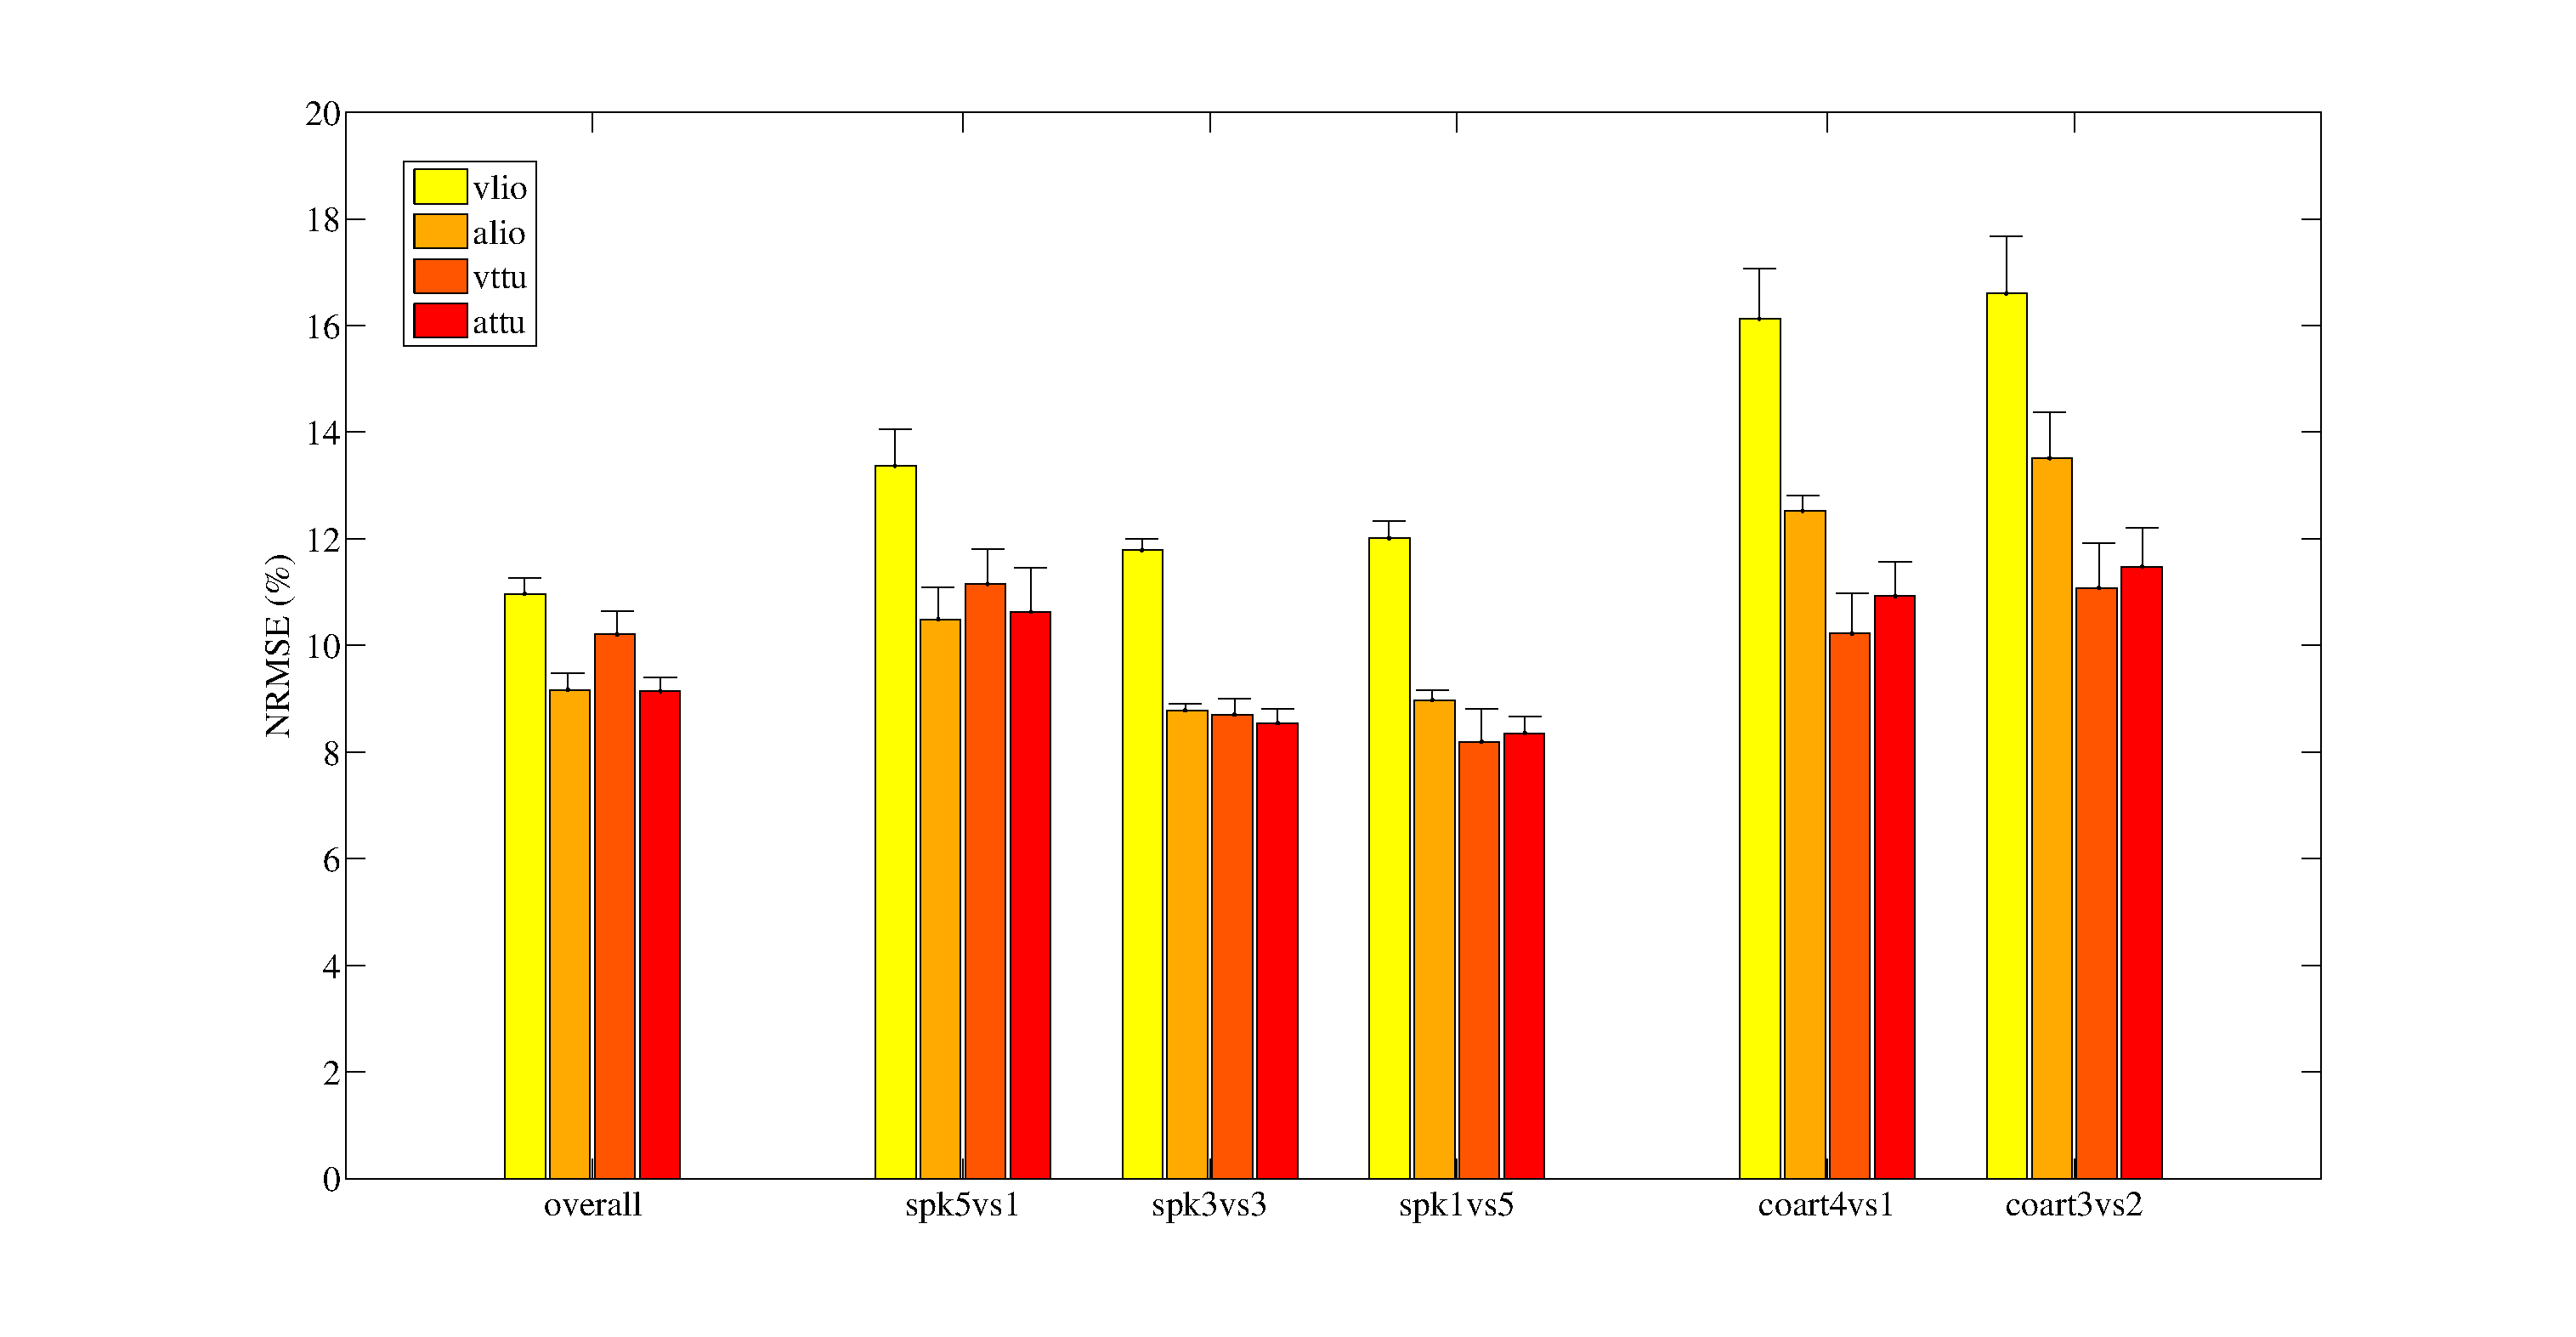
\includegraphics[width=\textwidth]{figs/AMM}}
  \caption{Quantitative performance of the AMM. For each cross-validation schema (overall, etc.)
    and output signal (\vlio, etc.) the NRMSE average value and standard error of the mean
    is reported.}
  \label{fig:amm_perf}
\end{figure*}

\begin{figure*}[t]
  \centerline{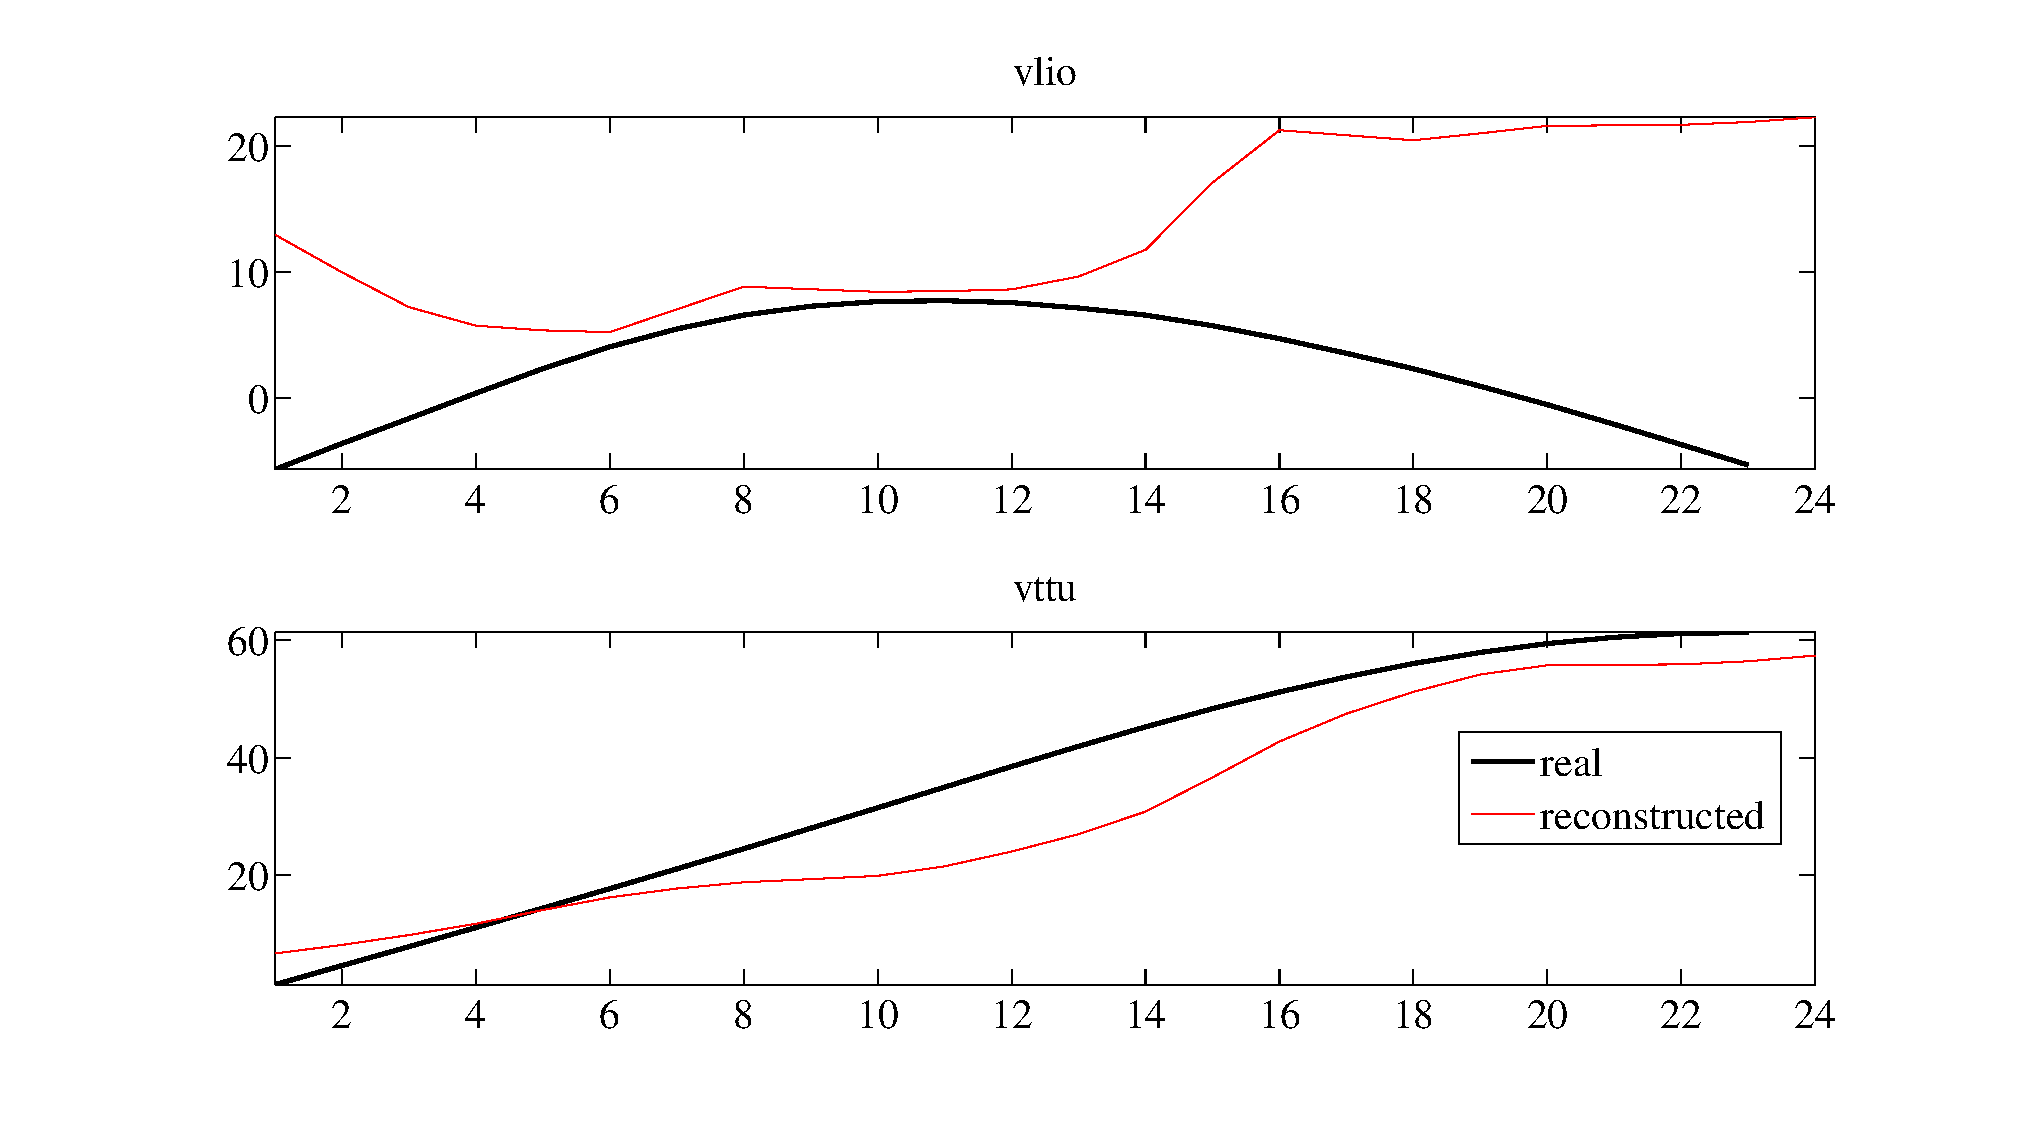
\includegraphics[width=\textwidth]{figs/recMIs}}
  \caption{Real and AMM-reconstructed \vlio\ and \vttu\ for subject $6$ uttering
    the /t/ in \emph{accento?} (accent). Notice the apparent gap in the quality
    of the reconstruction, favouring in this case the labiodental trajectory (\vttu).}
  \label{fig:example}
\end{figure*}

\begin{figure*}[t]
  \centerline{\includegraphics[width=\textwidth]{figs/doubleDiss}}
  \caption{Double dissociation of correlation between real and AMM-reconstructed MI
    (mean and standard error of the mean). Mean coefficients are significantly
    higher for \vlio\ when ``listening'' to labials than dentals ($0.8822 \pm 0.0119$
    versus $0.3381 \pm 0.0281$ with Student's t-test $p<0.01$) and vice-versa
    for \vttu\ ($0.9280 \pm 0.0096$ versus $0.5548 \pm 0.0236$, $p<0.01$). The \overall\ CV
    schema is used.}
  \label{fig:DD}
\end{figure*}

\begin{figure*}[t]
  \centerline{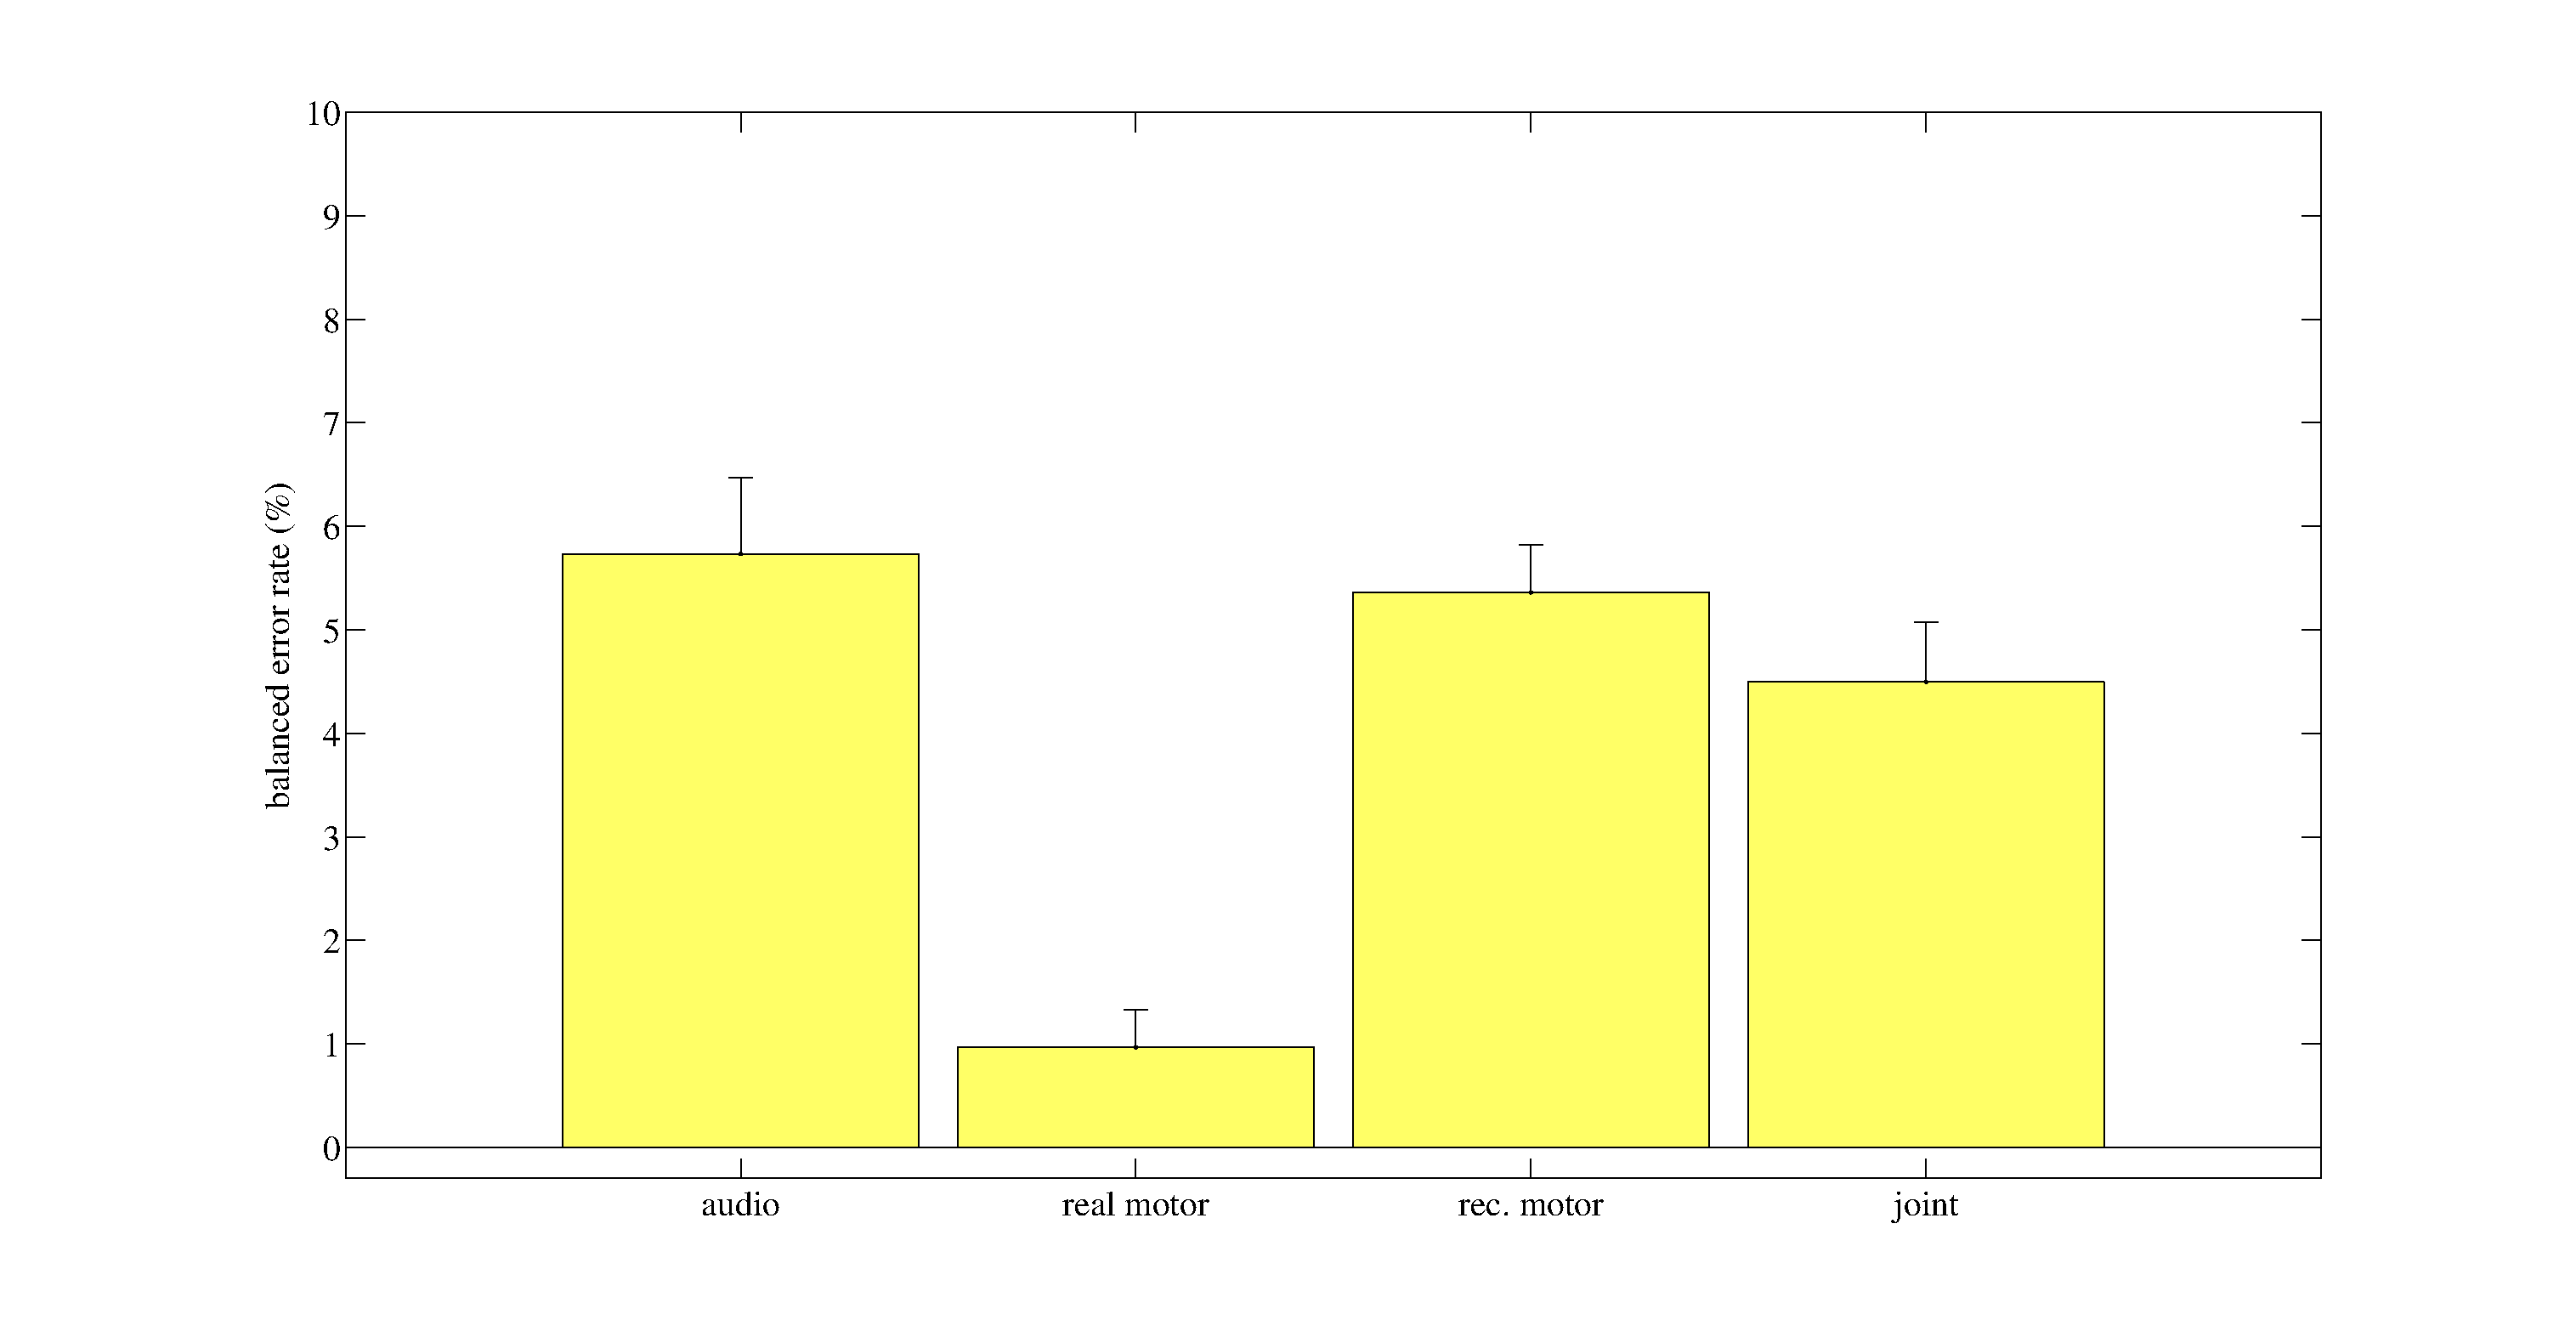
\includegraphics[width=\textwidth]{figs/exp1}}
  \caption{Balanced error rate in classification of bilabials and dentals obtained
    in the \overall\ CV schema, using audio features, real motor features,
    motor features reconstructed by the AMM, and by joining the audio and
    reconstructed-motor models.}
  \label{fig:class1_perf}
\end{figure*}

\begin{figure*}[t]
  \centerline{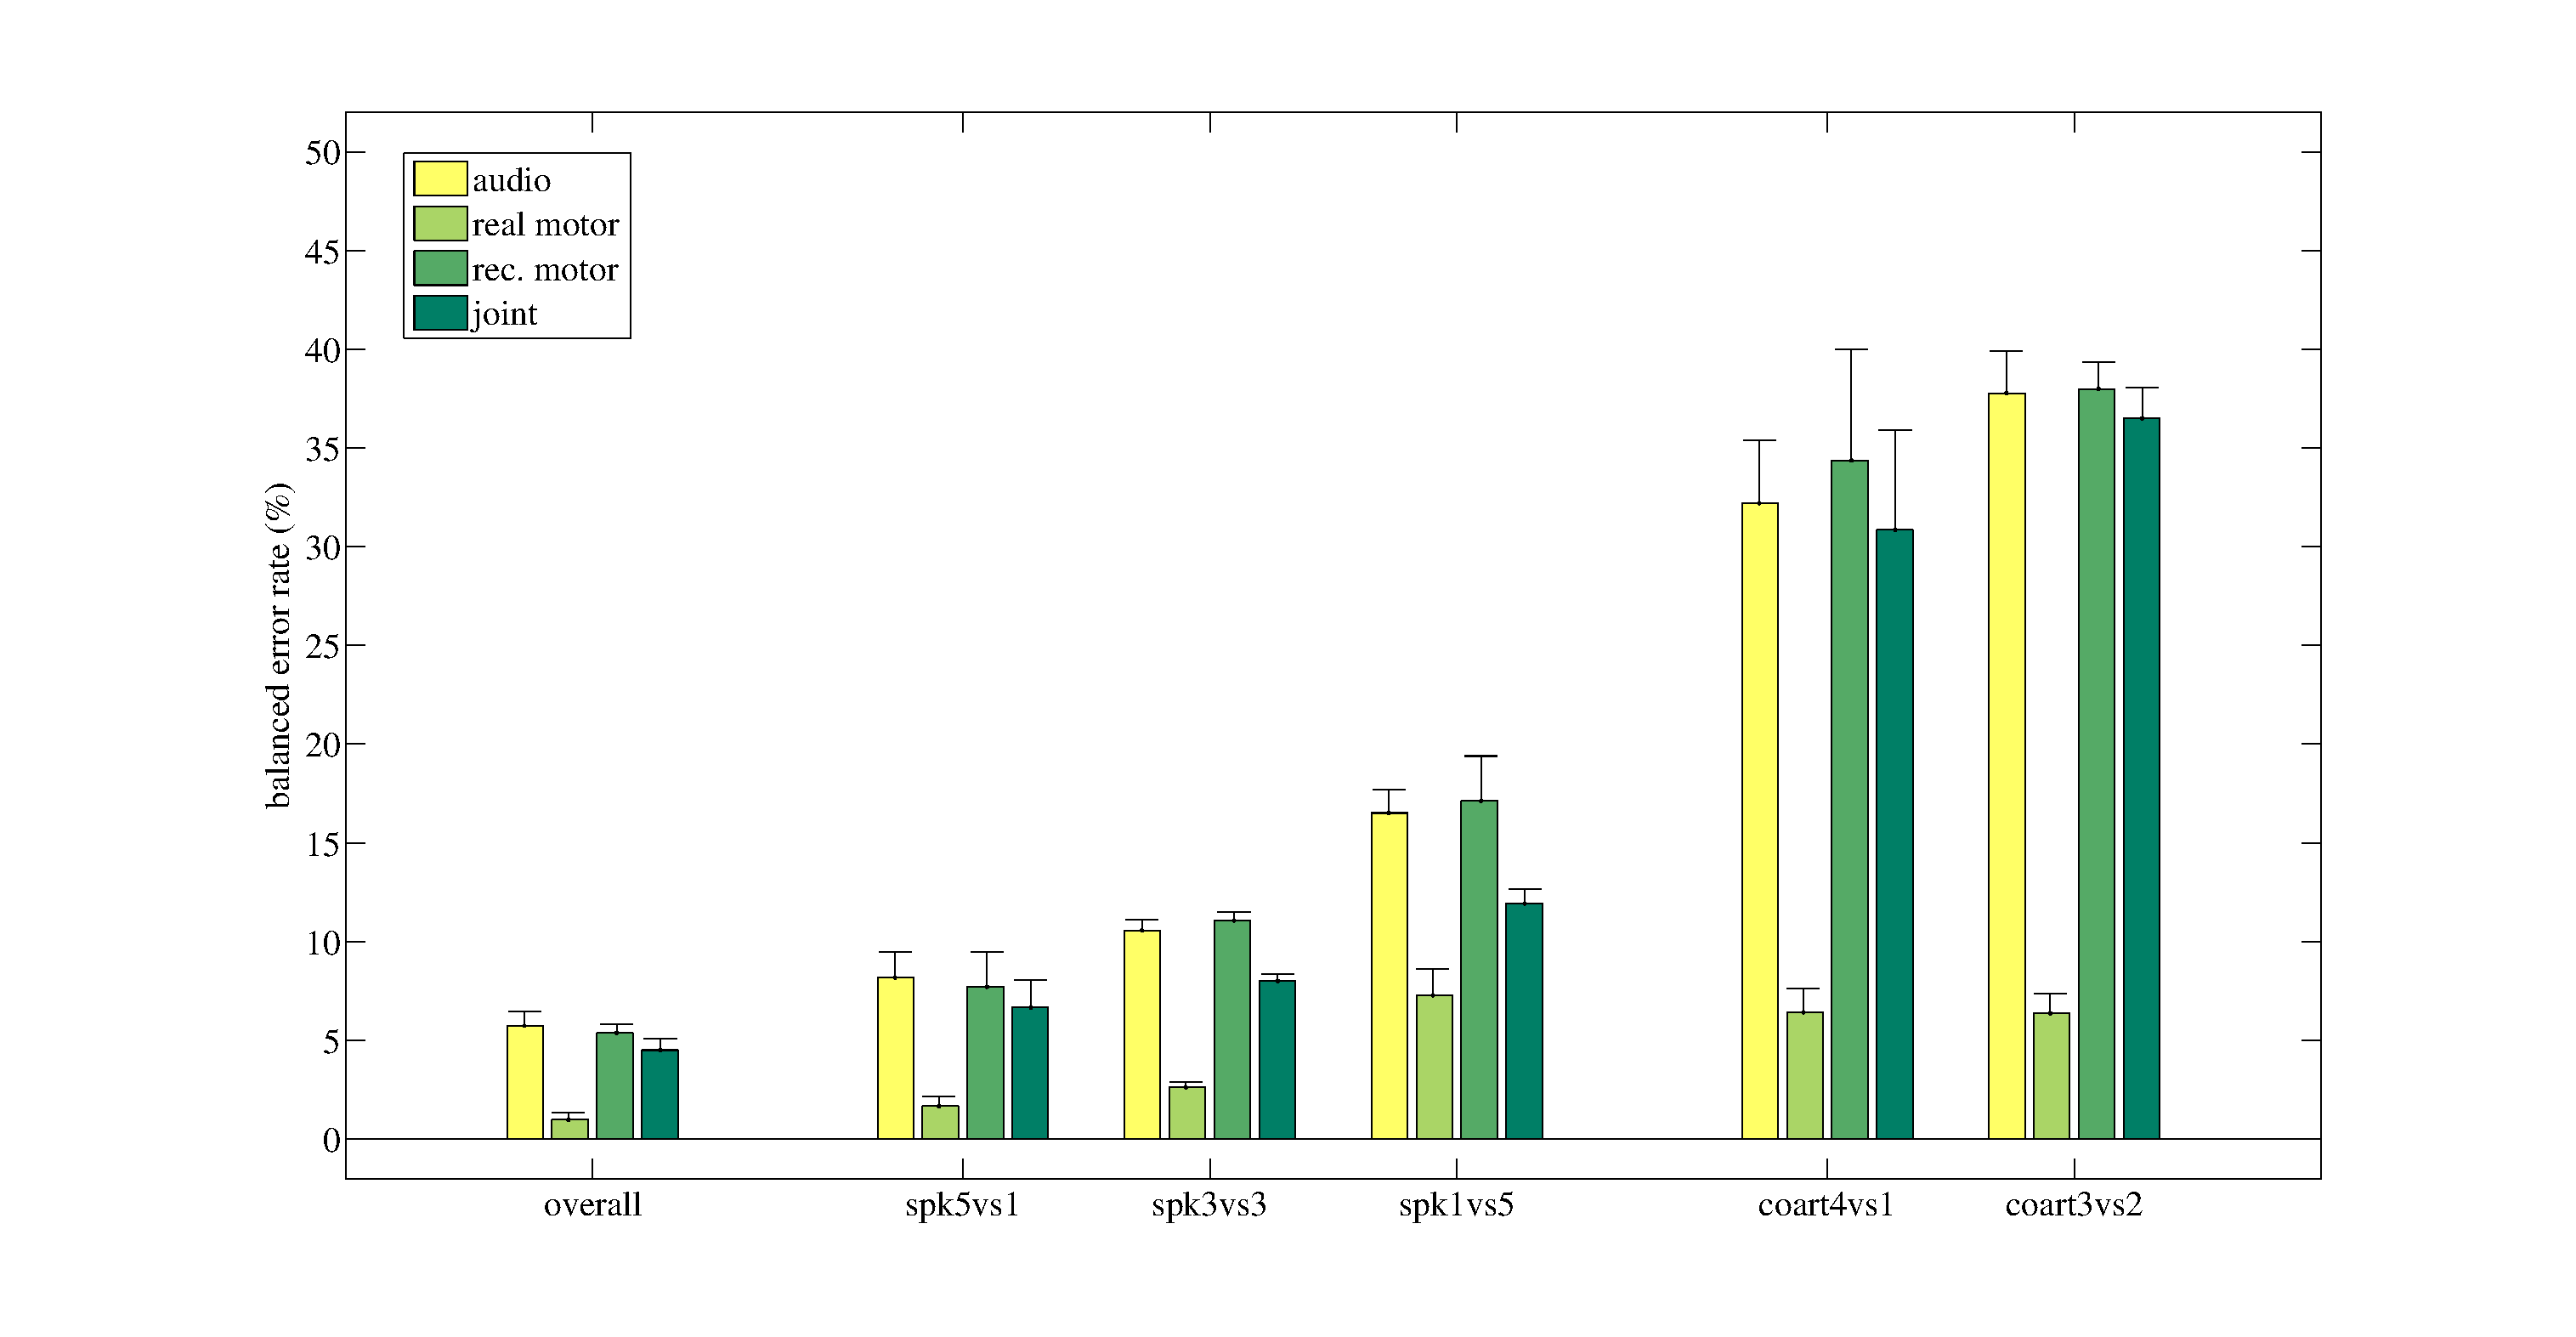
\includegraphics[width=\textwidth]{figs/exp2}}
  \caption{Balanced error rate in classification of bilabials and dentals for each
    CV schema, using the four sets of features of Figure \ref{fig:class1_perf}.}
  \label{fig:class2_perf}
\end{figure*}

\begin{figure*}[t]
  \centerline{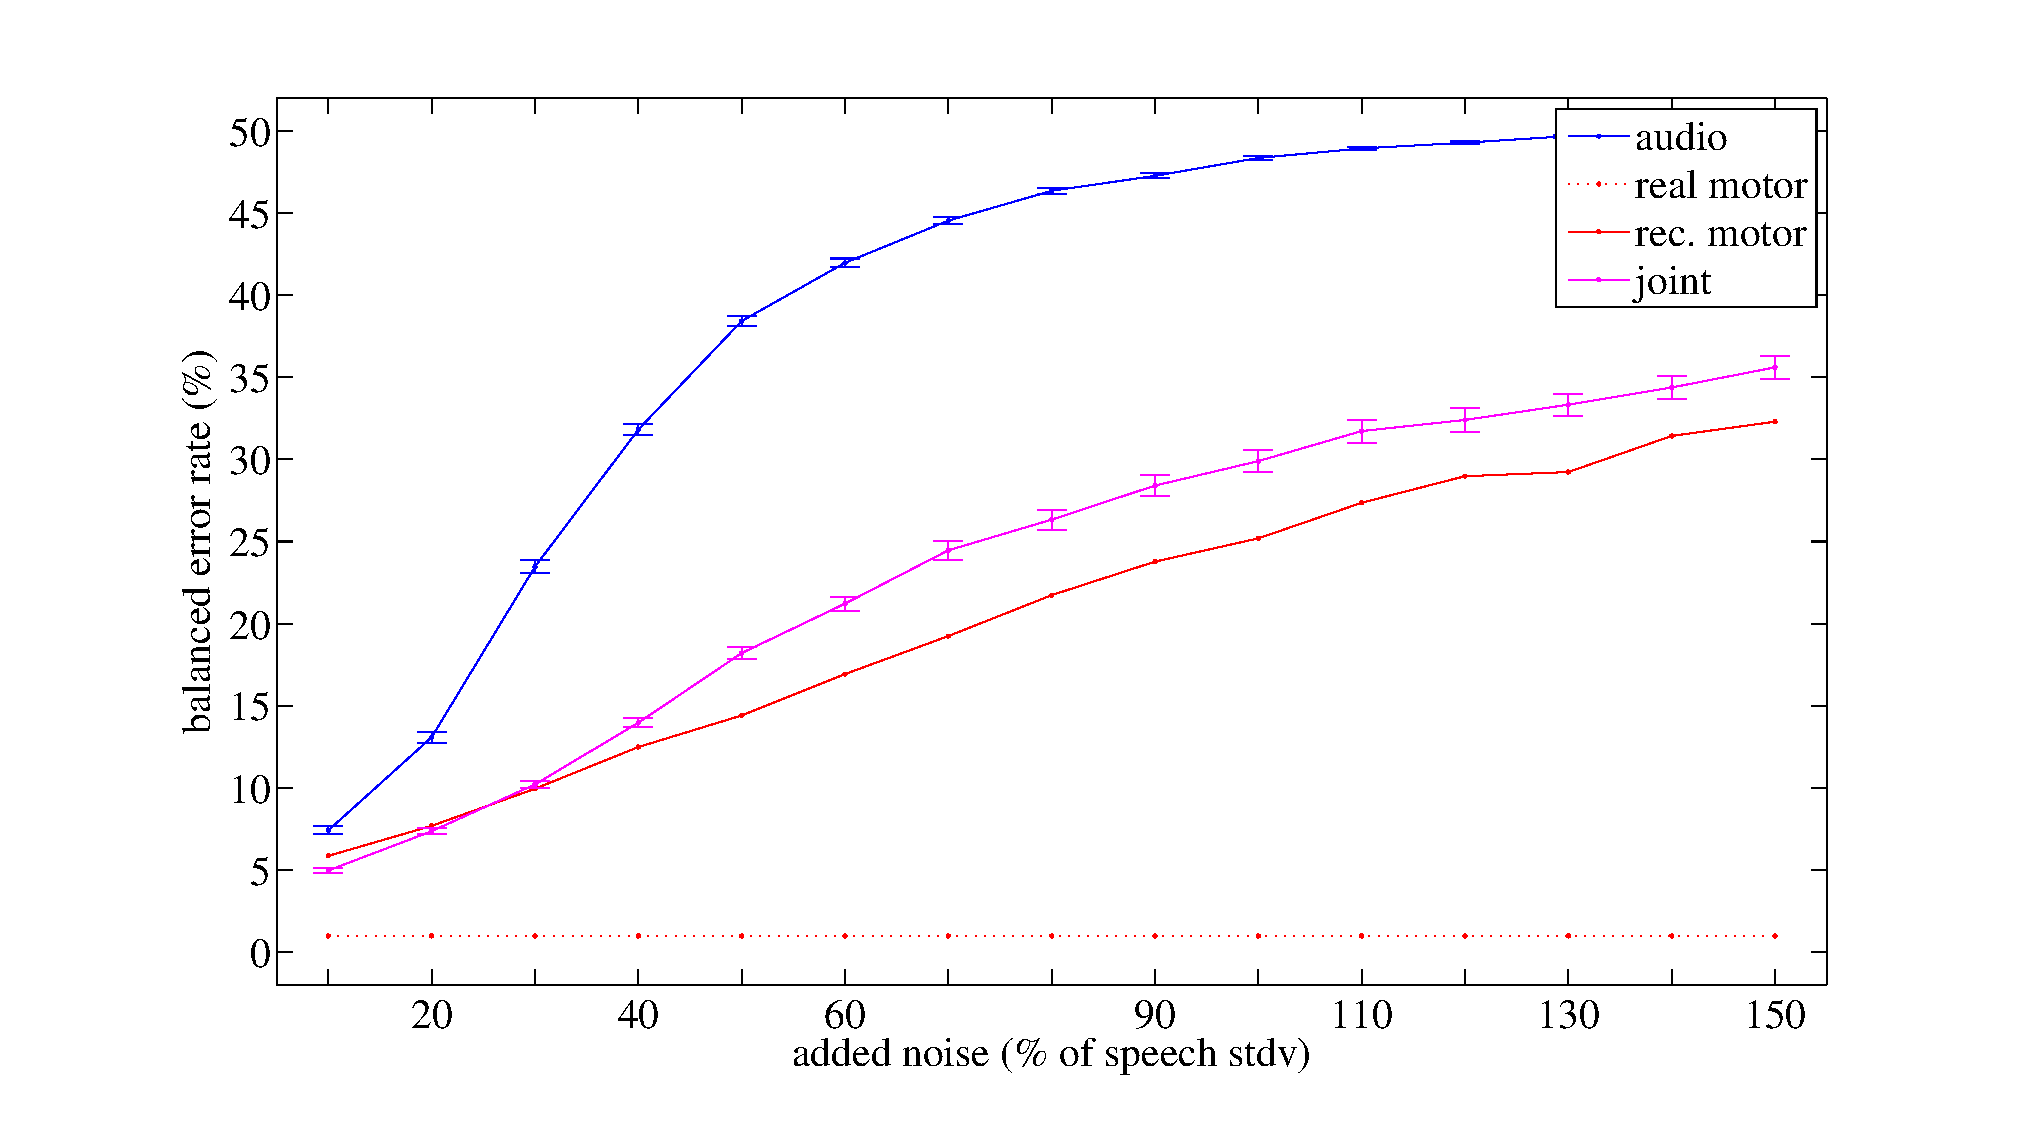
\includegraphics[width=\textwidth]{figs/exp3}}
  \caption{Balanced error rate in classification of bilabials and dentals for the
    \overall\ CV schema as noise is added, using the sets of features of Figure
    \ref{fig:class1_perf}.}
  \label{fig:class3_perf}
\end{figure*}

\end{document}
